% \iffalse The license starting three lines down applies to this file.
%<*batchfile>
{\obeylines\obeyspaces \gdef\thepreamble{

LaTeX package gradientframe for simple rectangular gradient frames around objects.

Copyright (C) Christian Raue, 2011
Send feedback to christian�raue@gmail�com (after being exposed to gravity).

This file may be distributed and/or modified under the
conditions of the LaTeX Project Public License, either
version 1.3c of this license or (at your option) any later
version.  The latest version of this license is in:

	http://www.latex-project.org/lppl.txt

and version 1.3c or later is part of all distributions of
LaTeX version 2005/12/01 or later.

This work has the LPPL maintenance status "maintained".

The Current Maintainer of this work is Christian Raue.

This work consists of gradientframe.dtx and the derived file
gradientframe.sty.

}}

\begingroup
%
% docstrip.cfg
%
% Sample configuration for the docstrip program for the ecv class
%

% BaseDirectory: To this directory the class will be installed
%\BaseDirectory{/usr/share/texmf}
\BaseDirectory{.}

% Path mapping for the directories defined in the ins file
%\DeclareDir{tex/latex/ecv}{tex/latex/ecv}
\DeclareDir{tex/latex/ecv}{.}

\keepsilent
\usedir{tex/latex/\jobname}
\expandafter\preamble\thepreamble\endpreamble
\askforoverwritefalse
\generate{\file{\jobname.sty}{\from{\jobname.dtx}{package}}}
\endgroup

\documentclass{ltxdoc}
\usepackage[american]{babel}
\usepackage[T1]{fontenc}
\usepackage{lmodern}
\usepackage{charter}
\usepackage[%
	inner=55mm,%
	outer=10mm,%
	top=20mm,%
	bottom=20mm,%
]{geometry}
\usepackage{color}
\usepackage[%
	pdftitle={the \jobname{} package},%
	pdfauthor={Christian Raue},%
	pdfsubject={LaTeX package documentation},%
	pdfkeywords={\jobname{} LaTeX rectangular gradient frame border around object table figure},%
 	pdfproducer={LaTeX},%
 	pdfcreator={LaTeX},%
	pdfborder={0 0 0},%
	pdfpagemode={UseOutlines},%
	pdfstartview={FitH},%
	pdfview={FitH},%
	pdfdisplaydoctitle=true,%
	]{hyperref}
\usepackage{tabularx}
\usepackage{listings}
\definecolor{lightgray}{gray}{.95}
\lstset{%
	frame=trbl,%
	framerule=0pt,%
	basicstyle=\footnotesize\ttfamily,%
	breaklines=true,%
	tabsize=4,%
	numbers=left,%
	numberstyle=\tiny,%
	backgroundcolor=\color{lightgray},%
}
\usepackage{emp}
\ifx\pdftexversion\undefined
	\usepackage[dvips]{graphicx}
\else
	\usepackage{graphicx}
	\DeclareGraphicsRule{*}{mps}{*}{}
\fi
\usepackage{\jobname}

\DoNotIndex{\def}

%\CodelineIndex
%\EnableCrossrefs
%\RecordChanges
%\OnlyDescription
%\setcounter{IndexColumns}{2}
\GetFileInfo{\jobname.sty}

\newcommand{\supdot}{%
	\scalebox{1.2}{$\dot{~}$}%
}
\newcommand{\package}[1]{%
	\texttt{#1}%
}
\newcommand{\resultarrow}{%
	\begin{center}
		\scalebox{2}{%
			\begin{picture}(9,10)
				\put(5,10){\vector(0,-4){10}}
			\end{picture}%
		}
	\end{center}%
}
\newcommand{\face}{%
	\begingroup
		\setlength{\fboxsep}{5px}%
		\scalebox{2}{\fbox{%
			\Huge
			$\ddot\smile$%
		}}%
	\endgroup
}
\newcommand{\command}[1]{%
	\texttt{\textbackslash{}#1}%
}

\title{the \package{\jobname} package\thanks{This document corresponds to \package{\jobname}~\fileversion, dated \filedate.}\\[1em]}
\author{Christian Raue\\[1em]\texttt{christian\supdot{}raue@gmail\supdot{}com}\\(after being exposed to gravity)\\[2em]}
\date{\filedate}

\begin{document}
\maketitle


\phantomsection
\addcontentsline{toc}{section}{\abstractname}
\begin{abstract}
\noindent
The \package{\jobname} package provides a command, \command{gradientframe}, for simple and discreet rectangular grayscale
gradient frames around objects, such as figures or tables, to set them apart from the surrounding text.
\end{abstract}


\phantomsection
\addcontentsline{toc}{section}{\contentsname}
\tableofcontents
\clearpage


\section{Introduction}
The \package{gradientframe} package is loaded in the usual way, i.e. by putting the line
\begin{quote}
	|\usepackage{gradientframe}|
\end{quote}
in the document's preamble. The \package{gradientframe} package depends on the \package{color} package which is loaded
by the \package{gradientframe} package if not already done so far in the document's preamble.


\section{Usage}
\DescribeMacro\gradientframe
To frame an object, such as figure, table, etc., use the \command{gradientframe\marg{object}} command.
By using \command{gradientframe\oarg{name=value,\ldots}\marg{object}}, the result can be influenced by providing the
following options by name:
\begin{itemize}
	\item
		\texttt{linewidth} (default value: \texttt{0.3px})\\
		defines each color's line width
	\item
		\texttt{padding} (default value: \texttt{0mm})\\
		defines space between the object and the frame (applies to all four sides)
\end{itemize}
Also take a look at the following examples.


\section{Examples}
\subsection{Frame surrounding a figure}
\begin{lstlisting}
	\begin{center}
		\gradientframe{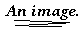
\includegraphics{image.jpg}}
	\end{center}
\end{lstlisting}
\resultarrow
\begin{center}
	\gradientframe{\face}
\end{center}


\subsection{Frame surrounding a figure with additional space}
\begin{lstlisting}
	\begin{center}
		\gradientframe[padding=5mm]{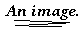
\includegraphics{image.jpg}}
	\end{center}
\end{lstlisting}
\resultarrow
\begin{center}
	\gradientframe[padding=5mm]{\face}
\end{center}


\subsection{Frame surrounding a figure with thicker frame lines and additional space}
\begin{lstlisting}
	\begin{center}
		\gradientframe[linewidth=1px,padding=5mm]{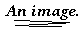
\includegraphics{image.jpg}}
	\end{center}
\end{lstlisting}
\resultarrow
\begin{center}
	\gradientframe[padding=5mm,linewidth=1px]{\face}
\end{center}


\subsection{Frame surrounding a table}
\begin{lstlisting}
	\begin{center}
		\gradientframe{%
			\begin{tabular}{r|l}
				\textbf{column A}	& \textbf{column B}	\\\hline
				cell 1A				& cell 1B			\\\hline
				cell 2A				& cell 2B			\\\hline
				cell 3A				& cell 3B			\\
			\end{tabular}%
		}
	\end{center}
\end{lstlisting}
\resultarrow
\begin{center}
	\gradientframe{%
		\begin{tabular}{r|l}
			\textbf{column A}	& \textbf{column B}	\\\hline
			cell 1A				& cell 1B			\\\hline
			cell 2A				& cell 2B			\\\hline
			cell 3A				& cell 3B			\\
		\end{tabular}%
	}
\end{center}
Be careful not to produce unintentional space when breaking lines. Add comments at line endings if needed to prevent
this, as shown in lines 2 and 8. Otherwise the result will look like this:
\begin{center}
	\gradientframe{
		\begin{tabular}{r|l}
			\textbf{column A}	& \textbf{column B}	\\\hline
			cell 1A				& cell 1B			\\\hline
			cell 2A				& cell 2B			\\\hline
			cell 3A				& cell 3B			\\
		\end{tabular}
	}
\end{center}


\clearpage
\subsection{Frame surrounding a MetaPost figure}
If you want to draw a frame around a MetaPost (or in the case of this example, MetaUML) generated figure, use the
\command{empuse} command.
\begin{lstlisting}
	\begin{center}
		\begin{empfile}
			\begin{empcmds}
				input metauml;
			\end{empcmds}
			\begin{empdef}[unique_name](0,0)
				save start, end;
				Begin.start;
				End.end;
				leftToRight(15)(start, end);
				drawObjects(start, end);
				clink(transition)(start, end);
			\end{empdef}
			\gradientframe[padding=5mm]{\empuse{unique_name}}
		\end{empfile}
	\end{center}
\end{lstlisting}
\resultarrow
\begin{center}
	\begin{empfile}
		\begin{empcmds}
			input metauml;
		\end{empcmds}
		\begin{empdef}[unique_name](0,0)
			save start, end;
			Begin.start;
			End.end;
			leftToRight(15)(start, end);
			drawObjects(start, end);
			clink(transition)(start, end);
		\end{empdef}
		\gradientframe[padding=5mm]{\empuse{unique_name}}
	\end{empfile}
\end{center}
Alternatively, you could outsource both, the \texttt{empdef} environment and the \command{empuse} command to a separate
file, and use \command{input\marg{filename}} as argument to the \command{gradientframe} command.


\section{Known issues}
\DescribeMacro\pagecolor
When using a page color different than white in combination with a (partially) transparent object, the transparent area
inside the frame will be white. To avoid this, a \command{colorbox} has to be drawn around the object. So instead of
\begin{quote}
	\command{pagecolor\marg{color}}\\
	\command{gradientframe\marg{object}}
\end{quote}
one should use
\begin{quote}
	\command{pagecolor\marg{color}}\\
	\command{gradientframe\{\command{colorbox}\marg{color}\marg{object}\}}
\end{quote}
This issue will hopefully be addressed in a future version.


\StopEventually{
	\typeout{****************************************************}
	\typeout{* To finish the installation, you have to move the}
	\typeout{* following file into a directory searched by TeX:}
	\typeout{*}
	\typeout{* \space\space \jobname.sty}
	\typeout{*}
	\typeout{* Documentation is in \jobname.\ifpdf pdf\else dvi\fi.}
	\typeout{*}
	\typeout{* Happy TeXing!}
	\typeout{****************************************************}
	\end{document}
}


\clearpage
\DocInput{\jobname.dtx}


\clearpage
%\phantomsection
%\addcontentsline{toc}{section}{Change history}
%\PrintChanges
\section{Change history}

\newlength{\notewidth}
\settowidth{\notewidth}{Note: }
\newcommand{\noteindent}{\hspace*{\notewidth}}
\begin{tabularx}{\textwidth}{|l|l|X|}
	\hline
	v0.1	& 2011/02/10	&	Initial version.
	\\\hline
	v0.1a	& 2011/02/10	&	Changed file encoding to ISO-8859-1 due to issues on CTAN.
	\\\hline
	v0.2	& 2011/02/13	&	Applied several code improvements.\newline
								Added key/value options for more flexibility.\newline
								Note: This breaks backward compatibility, so change calls in the form\newline
								\noteindent \command{gradientframe[\meta{width}]\marg{object}}\newline
								\noteindent to\newline
								\noteindent \command{gradientframe[padding=\meta{width}]\marg{object}}\newline
								\noteindent in case of an update from previous versions.
	\\\hline
\end{tabularx}


%\phantomsection
%\addcontentsline{toc}{section}{Index}
%\PrintIndex


\Finale
%</batchfile>
% \fi
%
% \section{Implementation}
%
%
% \subsection{Package header}
%	\begin{macrocode}
\NeedsTeXFormat{LaTeX2e}[1999/12/01]
\ProvidesPackage{gradientframe}[2011/02/13 v0.2 simple gradient frames around objects]
\RequirePackage{color}
\RequirePackage{keyval}
%    \end{macrocode}%^^A must be exactly 4 spaces
%
% \subsection{Options for the \command{gradientframe} command}
% The \package{keyval} package is used to handle options given to the \command{gradientframe} command by name. These
% options are:
% \begin{itemize}
%	\item \texttt{linewidth} -- defines each color's line width
%	\begin{macrocode}
\define@key{gradientframe}{linewidth}{%
	\newdimen\gradientframe@linewidth%
	\setlength{\gradientframe@linewidth}{#1}%
}%
%    \end{macrocode}%^^A must be exactly 4 spaces
%
%	\item \texttt{padding} -- defines space between the object and the innermost frame line
%	\begin{macrocode}
\define@key{gradientframe}{padding}{%
	\newdimen\gradientframe@padding%
	\setlength{\gradientframe@padding}{#1}%
}%
%    \end{macrocode}%^^A must be exactly 4 spaces
% \end{itemize}
%
%^^A \define@key{gradientframe}{outercolor}{}
%^^A \define@key{gradientframe}{innercolor}{}
%
% \begin{macro}{\gradientframe@defaults}
% The default values for these options are defined as follows:
%	\begin{macrocode}
\newcommand{\gradientframe@defaults}{%
	\setkeys{gradientframe}{%
		linewidth=0.3px,%
		padding=0mm%
	}%
}%
%    \end{macrocode}%^^A must be exactly 4 spaces
% \end{macro}
%
% \subsection{Commands}
% \begin{macro}{\gradientframe@origlinewidth}
% This dimension is used internally to preserve the original line width defined by \command{fboxrule}.
%	\begin{macrocode}
\newdimen\gradientframe@origlinewidth%
%    \end{macrocode}%^^A must be exactly 4 spaces
% \end{macro}
%
% \begin{macro}{\gradientframe@drawbox}
% This command uses two colors, for border and background, and draws one frame line.
%	\begin{macrocode}
\newcommand{\gradientframe@drawbox}[3]{%
	\fcolorbox[gray]{#1}{#2}{%
		#3%
	}%
}%
%    \end{macrocode}%^^A must be exactly 4 spaces
% \end{macro}
%
% \begin{macro}{\gradientframe}
% This command draws the grayscale gradient frame around objects. This is achieved by drawing multiple frame lines side
% by side, each with a slightly different color.
%	\begin{macrocode}
\newcommand{\gradientframe}[2][]{%
	\gradientframe@defaults% apply defaults
	\setkeys{gradientframe}{#1}%
%
	\begingroup% limit redefinitions to this block
		% backup original \fboxrule value
		\setlength{\gradientframe@origlinewidth}{\fboxrule}%
%
		\setlength{\fboxrule}{\gradientframe@linewidth}%
		\setlength{\fboxsep}{\gradientframe@linewidth}% space between frame and object
		\gradientframe@drawbox{.98}{.96}{%
			\gradientframe@drawbox{.94}{.92}{%
				\gradientframe@drawbox{.90}{.88}{%
					\gradientframe@drawbox{.86}{.84}{%
						\gradientframe@drawbox{.82}{.80}{%
							\gradientframe@drawbox{.78}{.76}{%
								\gradientframe@drawbox{.74}{.72}{%
									\setlength{\fboxrule}{\gradientframe@origlinewidth}% restore original \fboxrule value
									\setlength{\fboxsep}{\gradientframe@padding}%
									\gradientframe@drawbox{.70}{1}{#2}%
								}%
							}%
						}%
					}%
				}%
			}%
		}%
	\endgroup%
}%
%    \end{macrocode}%^^A must be exactly 4 spaces
% \end{macro}
%
\endinput
% \endinput
